%\documentclass[11pt, oneside]{article}  

%\usepackage{style-3yp} %this is the .sty file
%\lfoot{Enzia Schnyder} %your name in the footer

%\usepackage{wrapfig}
%\usepackage{float}
%table
%\usepackage{array}
%\newcolumntype{L}{>{\centering\arraybackslash}m{2.5cm}}
%\newcolumntype{K}{>{\centering\arraybackslash}m{1.5cm}}
%\newcolumntype{J}{>{\centering\arraybackslash}m{2.8cm}}
%\usepackage{multirow}

%\begin{document}

\section{Heat Exchangers}
\subsection{Introduction}

Within the plant, there are many different streams that need to be heated and cooled. By designing a network of heat exchangers, heat can be transferred between these streams, thus improving overall plant efficiency. The pinch analysis method described by Smith \cite{hexbook} \cite{lecture:hex} was be used to design the heat exchange network so that streams are matched most effectively. 

\subsection{Stream data}
The turbine system was excluded from the heat exchange network as it is only in use 5\% of the generation time and thus cannot provide any useful heating/cooling most of the time. Data was gathered about the incoming and outgoing streams from each major process unit and is summarised in Table \ref{tab:heatexdata}. Figure \ref{fig:heatexflow} also shows how these streams are linked to the process units in the plant.

The change in enthalpy $\Delta H$ from the inlet to the outlet of each of the streams was calculated using:
\begin{equation} \label{eq:heatex}
\Delta H = \dot{m} C_p (T_{in} - T_{out})
\end{equation}
where $\dot{m}$ is the mass flow rate, $C_p$ is the specific heat capacity and $T_{in}$ and $T_{out}$ are the temperatures at the inlet and outlet respectively. The product $\dot{m} C_p$ is the heat capacity flow rate denoted as $CP$. Negative changes in enthalpy correspond to hot streams that must be cooled (heat supply) and positive changes in enthalpy correspond to cold streams that must be heated (heat demand).

\begin{figure} [h]
\centering
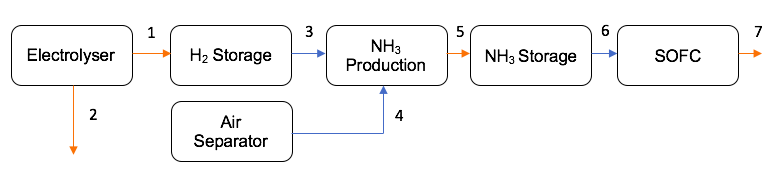
\includegraphics[width=0.99\textwidth]{./pictures/heatexflow.png}
  \caption{A diagram showing how different streams in the heat exchange network are related to the process units. Blue arrows represent cold streams that must be heated up and red arrows represent hot streams that must be cooled} \label{fig:heatexflow}
\end{figure}

\begin{table} [h]
\begin{center}
\caption{Data for streams coming in and out of all major process units of the ESS plant} \label{tab:heatexdata} 
\begin{tabular}{ |c|c|L|c|c|c|L| }
 \hline
Stream & Composition & $\dot{m} $ $(kg/s) $& $C_p$ $(kJ kg^{-1} K^{-1})$  & $T_{in}$ $(K)$ & $T_{out}$ $(K)$ & $\Delta H$ $(kW)$ \\ 
 \hline
  1 & $H_2$ & 0.4844 & 14.3 & 393 & 298 & -658\\ 
 \hline
 2 & $O_2$ & 35.75 & 0.919 & 393 & 298 & -3119\\ 
 \hline
3 & $H_2$ & 0.5099 & 14.3 & 298 & 473 & 1276\\
\hline
4 & $N_2$ & 2.34 & 1.04 & 288 & 473 & 450.2\\
 \hline
  5 & $NH_3$ & 2.795 & 2.19 & 238 & 233 &-30.6\\
 \hline
 6 & $NH_3$ & 2.655 & 2.19 & 233 & 243 & 58.1\\
 \hline
 7 & Air & 200 & 1.01 & 898 & 298 & -121200\\
 \hline
\end{tabular}
\end{center}  
\end{table}
Streams 2 and 7 are exhaust streams so they do not have to be fully cooled fully, and can be used as heating utilities with maximum power described in Table \ref{tab:heatexdata}. This results in a total heat demand of 4.54MW and a total heat supply of 0.689MW with additional 124MW provided by hot streams 2 and 7. Therefore heating power must be supplied from streams 2 or 7 to fulfill heating requirements, extra heat that is not required for the network can be used as part of a cogeneration system.

\subsection{Design Problem} \label{ssec:utility}

A problem table, shown in Table \ref{tab:problemtable}, was used to summarise the temperature difference in each stream and to find the change in enthalpy across each temperature interval. For this table, the actual stream temperatures were shifted to guarantee that each heat exchanger will operate over a minimum temperature difference $\Delta T_{min}$: $T_H^* = T_H - \frac{\Delta T_{min}}{2}$ for hot streams and $T_C^* = T_C + \frac{\Delta T_{min}}{2}$ for cold streams. A large $\Delta T_{min}$ means that less heat can be recovered, increasing utility costs. Decreasing $\Delta T_{min}$ will increase the heat recovered but will also increase the area of the heat exchangers required and the capital cost. It was set to 20K as the streams at the pinch points are gaseous, which require a larger $\Delta T_{min}$ than liquid streams \cite{hexbook}. Streams 2 and 7 were excluded from the problem table as they do not need to be cooled fully.

\begin{table} [h]
\begin{center}
\caption{Problem table for this design problem} \label{tab:problemtable} 
\renewcommand{\arraystretch}{0.95}
\begin{tabular}{ |c|c|c|c|c|c|c|c|c| }
 \hline
$T^*$ $(K)$ &  \multicolumn{5}{|c|}{Stream \& CP $(kWK^{-1})$} & \multirow{2}{*}{$\Delta T \ (K)$} & \multirow{2}{*}{$\Delta H_{int} \ (kW)$}\\  \cline{1-6}
   \multirow{2}{*}{483} & 1 - 6.93 & 3 - 7.29 & 4 - 2.43 & 5 - 6.12 & 6 - 5.81 & & \\ 
 \cline{2-8}
  & \multirow{2}{*}{} &\multirow{2}{*}{$\uparrow$} & \multirow{2}{*}{$\uparrow$}& \multirow{2}{*}{}&\multirow{2}{*}{} & \multirow{2}{*}{100} & \multirow{2}{*}{-972}\\ 
 \cline{1-1}
\multirow{2}{*}{383} & & & & & & &\\
\cline{2-8}
& \multirow{2}{*}{|} &\multirow{2}{*}{|} & \multirow{2}{*}{|}& \multirow{2}{*}{}&\multirow{2}{*}{} & \multirow{2}{*}{75} & \multirow{2}{*}{-209.3} \\ 
 \cline{1-1}
\multirow{2}{*}{308} & & & & & & &\\
\cline{2-8}
 & \multirow{2}{*}{|} &\multirow{2}{*}{} & \multirow{2}{*}{|}& \multirow{2}{*}{}&\multirow{2}{*}{} & \multirow{2}{*}{10} & \multirow{2}{*}{45}\\ 
 \cline{1-1}
 \multirow{2}{*}{298} & & & & & & &\\
\cline{2-8}
& \multirow{2}{*}{$\downarrow$} &\multirow{2}{*}{} & \multirow{2}{*}{}& \multirow{2}{*}{}&\multirow{2}{*}{} & \multirow{2}{*}{10} & \multirow{2}{*}{69.3} \\ 
 \cline{1-1}
 \multirow{2}{*}{288} & & & & & & &\\
\cline{2-8}
 & \multirow{2}{*}{} &\multirow{2}{*}{} & \multirow{2}{*}{}& \multirow{2}{*}{}&\multirow{2}{*}{} & \multirow{2}{*}{35} & \multirow{2}{*}{0}\\ 
 \cline{1-1}
 \multirow{2}{*}{253} & & & & & & &\\
\cline{2-8}
 & \multirow{2}{*}{}&\multirow{2}{*}{} & \multirow{2}{*}{}& \multirow{2}{*}{}&\multirow{2}{*}{$\uparrow$} & \multirow{2}{*}{10} & \multirow{2}{*}{-58.1}\\ 
 \cline{1-1}
 \multirow{2}{*}{243} & & & & & & &\\
\cline{2-8}
 & \multirow{2}{*}{}&\multirow{2}{*}{} & \multirow{2}{*}{}& \multirow{2}{*}{}&\multirow{2}{*}{} & \multirow{2}{*}{15} & \multirow{2}{*}{0}\\ 
 \cline{1-1}
 \multirow{2}{*}{228} & & & & & & &\\
  \cline{2-8}
 & \multirow{2}{*}{}&\multirow{2}{*}{} & \multirow{2}{*}{}& \multirow{2}{*}{$\downarrow$}&\multirow{2}{*}{} & \multirow{2}{*}{5} & \multirow{2}{*}{30.6}\\
 \cline{1-1}
 \multirow{2}{*}{223} & & & & & & &\\
 \cline{2-8}
&\multicolumn{7}{|c|}{}  \\
 \hline
\end{tabular}
\end{center}  
\end{table}

\begin{wrapfigure}{r}{0.48\textwidth}
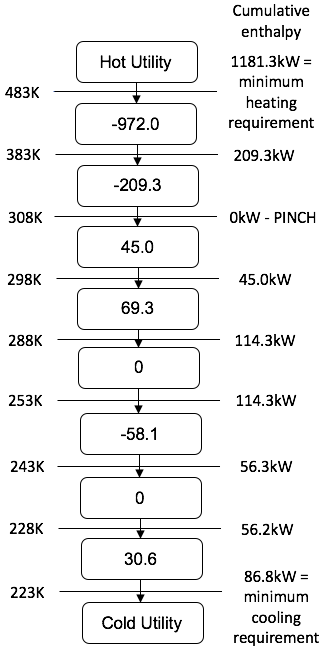
\includegraphics[width=0.9\linewidth]{./pictures/cascadediagram2} 
\caption{Cascade diagram for the heat exchange network.}
\label{fig:cascade}
\end{wrapfigure}
Using the problem table, the maximum cumulative negative enthalpy (greatest heat deficit) was -1181.3kW at 308K, the pinch point. This cannot be realised as it requires heat to be transferred up the temperature scale. To resolve this a hot utility of 1181kW was added. This heat cascades down the system to heat deficit intervals cooler in temperature as shown in Figure \ref{fig:cascade}. The cascade diagram shows that the minimum heating and cooling requirements needed to satisfy the problem are 1181.3kW and 86.8kW respectively.

\subsection{Pinch Design}
Using the pinch design method, two separate networks were independently designed above and below the pinch. This is because minimum utility requirements cannot be met if heat is transferred across the pinch. To satisfy all stream requirements, two constraints also have to be met:
\\ 1. Above the pinch, the number of hot streams must be less than or equal to the number of cold streams so that cooling utilities are not needed.
\\ 2. The heat capacity flow rate of hot streams must be less than or equal to that of the cold stream they are matched with, so that no point has a temperature difference less than $\Delta T_{min}$. 

The reverse constraints apply below the pinch and are summarised in Table \ref{tab:pinchconstraints}, which shows that the first constraint is not met above the pinch. Stream 1 was not hot enough to heat streams 3 and 4 so a fraction of stream 7 was added to the network to heat them (marked with *), which also allows the first constraint to be satisfied. Where there were multiple streams that can be matched, they were selected to give the greatest temperature difference, which reduces area of the heat exchangers and therefore the capital cost of the network required. Equation \ref{eq:heatex} was used to calculate enthalpy requirements and temperature coming out of each heat exchanger.

\begin {table} [h]
\begin{center}
\caption{Constraints for pinch design of the heat exchange network. The top half of the table describes design constraints and the bottom half shows stream data. Hot streams are colored red and cold streams are colored blue.} \label{tab:pinchconstraints} 
\begin{tabular}{ |K|K|K|K|K|K|K|K| }
 \hline
\multicolumn{4}{|c|}{Above pinch} & \multicolumn{4}{|c|}{Below pinch}\\
\hline
\multicolumn{4}{|c|}{$N_H \leqslant N_C$} & \multicolumn{4}{|c|}{$N_H \geqslant N_C$}\\
 \hline
\multicolumn{4}{|c|}{ $CP_H \leqslant CP_C$} & \multicolumn{4}{|c|}{$CP_H \geqslant CP_C$}\\
 \hline
  \textcolor{red}{S1} &\textcolor{red}{6.93} & \textcolor{blue}{S3} & \textcolor{blue}{7.29} & \textcolor{red}{S1} & \textcolor{red}{6.93} & \textcolor{blue}{S4} & \textcolor{blue}{2.43}\\
  \hline
  \textcolor{red}{S7*}& \textcolor{red}{2.04}& \textcolor{blue}{S4} & \textcolor{blue}{2.43} & \textcolor{red}{S5} & \textcolor{red}{6.12} & \textcolor{blue}{S6} &  \textcolor{blue}{5.81}\\
  \hline
\end{tabular}
\end{center}  
\end {table}

Above the pinch, stream 1 was fully cooled using stream 3. Streams 3 and 4 both then required further heating utility in the form of stream 7. The flow rate of stream 7 must be less than $2.4 kg s^{-1}$ to satisfy constraint 2 and was chosen to exactly satisfy the heating requirements of streams 3 and 4 while arriving at the pinch temperature resulting in a mass flow rate of $2.02 kg s^{-1}$. In total three heat exchangers were required: one as part of the main work and two as `heating utility' from stream 7. 

Below the pinch, stream 5 required cooling utility as no cold streams were cold enough to cool it. This left stream 1 to heat both streams 4 and 6. Stream 4 had a greater heating requirement so it was satisfied first. Stream 1 also requires cooling utility to remove the remaining heat. In total two heat exchangers and two cooling units were required. The full network is shown in Figure \ref{fig:heatexnetwork}, heat transferred across heat exchangers and utilities are also shown in Table \ref{tab:powerhex}. Stream 2 was not needed for the final design as enough heating power was provided by stream 7. 

\begin{figure} [h]
\centering
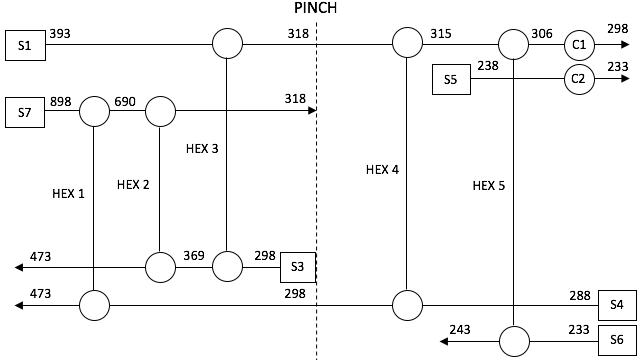
\includegraphics[width=0.85\textwidth]{./pictures/heatexnetworkBIG.png}
  \caption{The final heat exchange network. Each pair of circles represents a heat exchanger, single circles represent cooling utility and temperatures (K) are shown at each isothermal segment.} \label{fig:heatexnetwork}
  \end{figure}

\begin {table} [h]
\begin{center}
\caption{Heat transferred in all heat exchangers and utilities in the network} \label{tab:powerhex} 
\begin{tabular}{ |c|c|c|c|c|c|c|c|c| }
 \hline
  Component & HEX 1 & HEX 2 & HEX 3 & HEX 4 &HEX 5 & C1 & C2\\ 
 \hline
 heat transferred (kW) & 425.3 & 756.0 & 519.8 & 24.3 & 58.1 & 56.2 & 30.6\\ 
 \hline
\end{tabular}
\end{center}  
\end {table}

From Table \ref{tab:powerhex}, five heat exchangers and two cooling utility units were required. The total cooling utility required was 86.8kW and the total heating utility (in the form of stream 7) was 1181.3kW. This matches the minimum utility requirements calculated in Section \ref{ssec:utility}, which shows that the heat exchanger network is one of the optimal configurations that can be designed.

Streams 1, 6 and 7 in the network have variable flow rates. This means that to satisfy stream requirements at all times, there will occasionally have to be heat transferred across the pinch, increasing the utility requirements. A control system would have to be designed to adjust the mass flow rates of stream 7 and cooling water used for C1 and C2 according to the varying demand.

\subsection{Costing}
From section \ref{LM23}, the capital cost of a heat exchanger varies with heat exchange area $A (m^2)$ as:
\setlength{\belowdisplayskip}{1pt} \setlength{\belowdisplayshortskip}{1pt}
\setlength{\abovedisplayskip}{1pt} \setlength{\abovedisplayshortskip}{1pt}
\begin{equation} 
\mathrm{Cost \ (Million\ \$)} = 130 \frac{A}{0.093}^{0.78}
\end{equation}

The area of each heat exchanger was found using $Q = UA\Delta T_{LM}$
Where $Q$ is the heat transferred, $U$ is the overall heat transfer coefficient and $\Delta T_{LM}$ is the log-mean temperature difference across the heat exchanger. Due to the relatively small cost of the heat exchange network compared to the rest of the plant, approximate values for $U$ were taken from existing data assuming that all heat exchangers operate with gases to give $U=30Wm^{-2}$ \cite{hexcoeff}. The cost of the final network was \$241,000. 

\subsection{Conclusion}
This chapter shows that the heat exchanger network satisfies all of the heating and cooling requirements in the plant and is a cost effective and reliable way to increase plant efficiency by reducing utility requirements from 5.2MW to 86.8kW.

\bibliography{./turbine/heatexreport}
%
\bibliographystyle{unsrt}
%\printbibliography[heading=subbibliography]
%\end{document}